\begin{figure*}[t]
	\centering
	\addtolength{\tabcolsep}{-4.5pt}
	\begin{tabular}{ccccccccc}
		target & sample-1 & sample-2 & sample-3 & & target & sample-1 & sample-2 & sample-3
		\\
		\begin{overpic}[width=\resultwidth]{fig5/1_bump_1/target.jpg}
			\imglabel{Bump-1}
		\end{overpic} &
		\includegraphics[width=\resultwidth]{fig5/1_bump_1/good1.jpg} &
		\includegraphics[width=\resultwidth]{fig5/1_bump_1/good2.jpg} &
		\includegraphics[width=\resultwidth]{fig5/1_bump_1/bad1.jpg} &
		&
		\begin{overpic}[width=\resultwidth]{fig5/1_bump_2/target.jpg}
			\imglabel{Bump-2}
		\end{overpic} &
		\includegraphics[width=\resultwidth]{fig5/1_bump_2/good1.jpg} &
		\includegraphics[width=\resultwidth]{fig5/1_bump_2/good2.jpg} &
		\includegraphics[width=\resultwidth]{fig5/1_bump_2/bad1.jpg}
		\\
		\begin{overpic}[width=\resultwidth]{fig5/2_leather_1/target.jpg}
			\imglabel{Leather-1}
		\end{overpic} &
		\includegraphics[width=\resultwidth]{fig5/2_leather_1/good1.jpg} &
		\includegraphics[width=\resultwidth]{fig5/2_leather_1/good2.jpg} &
		\includegraphics[width=\resultwidth]{fig5/2_leather_1/bad1.jpg} &
		&
		\begin{overpic}[width=\resultwidth]{fig5/2_leather_2/target.jpg}
			\imglabel{Leather-2}
		\end{overpic} &
		\includegraphics[width=\resultwidth]{fig5/2_leather_2/good1.jpg} &
		\includegraphics[width=\resultwidth]{fig5/2_leather_2/good2.jpg} &
		\includegraphics[width=\resultwidth]{fig5/2_leather_2/bad1.jpg}
		\\
		\begin{overpic}[width=\resultwidth]{fig5/3_plaster_1/target.jpg}
			\imglabel{Plaster-1}
		\end{overpic} &
		\includegraphics[width=\resultwidth]{fig5/3_plaster_1/good1.jpg} &
		\includegraphics[width=\resultwidth]{fig5/3_plaster_1/good2.jpg} &
		\includegraphics[width=\resultwidth]{fig5/3_plaster_1/bad1.jpg} &
		&
		\begin{overpic}[width=\resultwidth]{fig5/3_plaster_2/target.jpg}
			\imglabel{Plaster-2}
		\end{overpic} &
		\includegraphics[width=\resultwidth]{fig5/3_plaster_2/good1.jpg} &
		\includegraphics[width=\resultwidth]{fig5/3_plaster_2/good2.jpg} &
		\includegraphics[width=\resultwidth]{fig5/3_plaster_2/bad1.jpg}
		\\
		\begin{overpic}[width=\resultwidth]{fig5/4_flake_1/target.jpg}
			\imglabel{Metallicflake-1}
		\end{overpic} &
		\includegraphics[width=\resultwidth]{fig5/4_flake_1/good1.jpg} &
		\includegraphics[width=\resultwidth]{fig5/4_flake_1/good2.jpg} &
		\includegraphics[width=\resultwidth]{fig5/4_flake_1/bad1.jpg} &
		&
		\begin{overpic}[width=\resultwidth]{fig5/4_flake_2/target.jpg}
			\imglabel{Metallicflake-2}
		\end{overpic} &
		\includegraphics[width=\resultwidth]{fig5/4_flake_2/good1.jpg} &
		\includegraphics[width=\resultwidth]{fig5/4_flake_2/good2.jpg} &
		\includegraphics[width=\resultwidth]{fig5/4_flake_2/bad1.jpg}
		\\
		\begin{overpic}[width=\resultwidth]{fig5/5_metal_1/target.jpg}
			\imglabel{Brushmetal-1}
		\end{overpic} &
		\includegraphics[width=\resultwidth]{fig5/5_metal_1/good1.jpg} &
		\includegraphics[width=\resultwidth]{fig5/5_metal_1/good2.jpg} &
		\includegraphics[width=\resultwidth]{fig5/5_metal_1/bad1.jpg} &
		&
		\begin{overpic}[width=\resultwidth]{fig5/5_metal_2/target.jpg}
			\imglabel{Brushmetal-2}
		\end{overpic} &
		\includegraphics[width=\resultwidth]{fig5/5_metal_2/good1.jpg} &
		\includegraphics[width=\resultwidth]{fig5/5_metal_2/good2.jpg} &
		\includegraphics[width=\resultwidth]{fig5/5_metal_2/bad1.jpg}
		\\
		\begin{overpic}[width=\resultwidth]{fig5/6_wood_1/target.jpg}
			\imglabel{Wood-1}
		\end{overpic} &
		\includegraphics[width=\resultwidth]{fig5/6_wood_1/good1.jpg} &
		\includegraphics[width=\resultwidth]{fig5/6_wood_1/good2.jpg} &
		\includegraphics[width=\resultwidth]{fig5/6_wood_1/bad1.jpg} & &
		\begin{overpic}[width=\resultwidth]{fig5/6_wood_2/target.jpg}
			\imglabel{Wood-2}
		\end{overpic} &
		\includegraphics[width=\resultwidth]{fig5/6_wood_2/good1.jpg} &
		\includegraphics[width=\resultwidth]{fig5/6_wood_2/good2.jpg} &
		\includegraphics[width=\resultwidth]{fig5/6_wood_2/bad1.jpg}
	\end{tabular}
	\captionsetup{labelfont=bf,textfont=it}
	\caption{\label{fig:fig5}
		\textbf{Results} of our MCMC sampling on \textbf{fig5etic} inputs. Each row corresponds to two examples of a different material model. For each example, the first column is the fig5etic target image. We show MCMC samples in the other columns, where sample-1 and sample-2 are chosen closer to the peak of the posterior distribution, and sample-3 is further away. More results please refer to supplemental materials.
	}
\end{figure*}
